\documentclass{article}

% Gestion des fonts
\usepackage[utf8]{inputenc}
%\usepackage[T1]{fontenc}

% Langue de rédaction
\usepackage[french]{babel}

% Gestion des images
\usepackage{graphics}
\graphicspath{{./Images/},{./Images/plot/}}

\DeclareGraphicsExtensions{.pdf,.png,.jpg}

% Gestion de l'esthètique
\usepackage[textwidth=0.7\paperwidth, textheight=0.7\paperheight]{geometry}

% Gestion des espaces
\usepackage{xspace}

% Commandes utilisateurs
\newcommand{\alinea}{\setlength{\parindent}{1cm}}
\newcommand{\abaqus}{\bsc{Abaqus}\xspace}
\renewcommand{\listfigurename}{Liste des figures}
% Bibliographie
% \bibitem[label 1]{cle 2} Auteur 3, TITRE 4, editeur 5, annee 6
%\renewcommand{\bibitem}[6]{\bibitem[#1]{#2} \textsc{#3}, \emph{#4}, #5, #6}


% Page de garde
\title{Compte-rendu du BE Butée offshore}
\author{\bsc{Muller} Marc \and \bsc{Buquet} Joseph}

\begin{document}
\maketitle

\newpage

\section{Abstract}

\section{Introduction}

%TODO Justification de la raideur transverse
% Explication de l'isogonflement lors de l'ajout de rondelles de métal

%TODO Raideur initiale
% Objectif 954 x 4 = 3816 N/cm

%TODO Justification choix lamelle
% Rayon identique à l'élastomère ou supérieur

\section{Approche du problème}

%TODO Unités utilisées
\begin{tabular}{|l|c|}
\hline
Unités & Dimensions \\ \hline
Longueur & cm \\
Pression & k Pa \\
Force & N \\
Raideur & N\/cm \\ \hline
\end{tabular}

\subsection{Butée offshore}
% taille, forme
% compression
% materiau
La butée offshore étudiée est une butée cylindrique de rayon $R_0 = 70 cm$ et de hauteur $H_0 = 100 cm$ en Chloroprène X10. Dans le cadre de cette étude, la butée va être soumise à une compression afin d'évaluer sa raideur à une flèche de $\Delta H = 30 cm$.

Pour ce faire, une modélisation numérique de celle-ci va être faite sous \abaqus. Dans ce contexte, les hypothèses suivantes seront avancées :
\begin{itemize}
\item Matériau isotrope
\item Symétrie axiale
La géométrie axiale de la pièce est cylindrique. Le matériau est de plus isotrope. Enfin la contrainte de compression est homogène sur la surface supérieure de la pièce et agit parallèlement à l'axe de symétrie de la pièce.
\item Modélisation du matériau
Il est demandé de travailler avec une loi hyperélastique de type Mooney-Rivlin, les détails de cette approximation seront approfondis par la suite.
\end{itemize}

\subsection{Choix des paramètres de Mooney-Rivlin}

Il a été demandé pour ce travail d'utiliser une loi hyperélastique de type Mooney-Rivlin. Pour la mettre en place, deux résultats de test expérimentaux sont utilisés (cf. figure~\ref{fig:essais_exp} : 
\begin{itemize}
\item un test de traction uniaxiale
Ce test est réalisé sur une éprouvette de longueur nominale $25 mm$ et de section nominale $8 mm^2$ selon une plage de déplacement de $0$ à $104 mm$.
\item un test de traction plane
Ce test est réalisé sur une éprouvette de hauteur nominale $35 mm$ et de section nominale $392 mm^2$ selon une plage de déplacement de $0$ à $57.5 mm$.
\end{itemize}

\begin{figure}
%\usegraphics{test_traction_uniaxiale}
\caption{Traction uniaxiale}
%\usegraphics{test_traction_plane}
\caption{Traction plane}
\label{fig:essais_exp}
\end{figure}

Ces deux essais ont permit d'obtenir deux courbes de réponses en effort-déplacement (cf. figure~\ref{fig:plot_donnees_essais}). A partir de ces courbes, une approximation des coefficients de Mooney-Rivlin est lancée sur \abaqus. Les tables de points résultant des essais sont pour cela entrés dans \abaqus et une évaluation automatique des coefficients est lancée. Il en résulte les coefficients lus dans le tableau~\ref{tab:donnees_MR}. Ceux-ci sont bien évidemment à mettre en face de ceux données lors du début de ce projet comme référence pour mettre en exergue la forte influence de l'approximation faite dans ce cadre.

\begin{tabular}{|l|c|c|c|}
% Les notres : C10 0.2499 C01 0.0942 D1 0.0584
% Les siennes: C10 0.043  C01 0.495  D1 0.000658
\hline
 & C10 & C01 & D1 \\ \hline
Valeurs évaluées & 0.2499 & 0.0942 & 0.0584 \\ \hline
Valeurs données & 0.043  & 0.495 & 0.000658 \\ \hline
\label{tab:donnees_MR}
\end{tabular} 

Pour rester en cohérence avec les résultats obtenus à l'aide d'\abaqus, il sera choisit de conserver les valeurs dites évaluées comme coefficients de Mooney-Rivlin pour notre matériau. Nous justifions ce choix par la courbe~\ref{fig:plot_donnees_essais} qui synthétise les données expérimentales et les réponses force-déplacement obtenus avec les coefficients de Mooney-Rivlin.

\begin{figure}
%\usegraphics{plot_donnees_essai}
\caption{Approximation du comportement du Chloroprène X10 par Mooney-Rivlin}
\label{fig:plot_donnees_essais}
\end{figure}

Afin d'étayer le choix de la méthode de Mooney-Rivlin dans cette étude, il est choisit de rappeler cette méthode.

\subsection{Explication de la méthode de Mooney-Rivlin}
%TODO écriture tensorielle
La méthode de Mooney-Rivlin est une méthode permettant de modéliser le potentiel élastique (ou de l'énergie de contrainte) d'un matériau. Pour cela, il est choisit une dépendance du potentiel élastique suivant les déviateurs des invariants $I_1$,$I_2$ du tenseur $B = V x V$ de Cauchy-Green gauche définit tel que $I_1 = Trace(B)$, $I_2 = \sec(B)$, $I_3=\det(\sigma)$.
On remarque que l'invariant $I_3$ n'est pas compris dans ce modèle. En effet, pour les élastomères, nous travaillons avec un effet Poisson $\nu = 0.49$, c'est-à-dire à volume quasi-constant. L'invariant $I_3$ est donc égal à 1 et n'est donc pas intéressant pour la modélisation de notre matériau puisqu'il n'évolue pas.

La méthode de Mooney-Rivlin résulte de l'amélioration du potentiel élastique de Mooney (1940) par Rivlin (1948) et statut la relation suivante \cite{wiki_MR}: $W = C_10(I_1-3) + C_01(I_2-3) + C_11(I_1-3)(I_2-3)$.
%TODO Corriger MR par l'ajout de barre sur les invariants.

De part l'expérience heuristique, il est assumé que cette approximation convient particulièrement bien dans la définition de l'hyperélasticité des elastomères spécialement sur des plages inférieure à 100\% de déformation en traction uniaxiale \cite{msc}.
%TODO avantages-inconvénients de MR
%Le modèle de Mooney-Rivlin peut être vu comme un cas particulier du modèle Ogden.

\subsection{Contact}
Lors de la compression de la butée offshore, l'élastomère se déforme à tel point que ses faces latérales viennent entrer en contact soit avec une lamelle d'acier ou avec lui-même. Dans ce cas, il faut définir une loi de contact pour éviter des problèmes d'interpénétration de la matière et obtenir des résultats convenables.

Dans cette étude, deux types de contact sont définis :
\begin{itemize}
\item le contact liant les parties aciers à l'élastomère
\item le contact pour les faces latérales de l'élastomère
\end{itemize}

Le premier contact est un contact de type \bsc{Tie} dans \abaqus, l'hypothèse est faite que l'interface entre la plaque d'acier et l'élastomère peut être considérée comme un encastrement. De manière classique, le maintien en position d'un élastomère et d'un acier est réalisé par une colle. Il est donc supposé que cette colle située à l'interface de nos deux pièces est rigides et qu'elle ne permet pas le mouvement des pièces ni en traction ni en cisaillement. Dans le cadre de cette étude où le comportement de notre élastomère est caractérisé en compression, il est raisonnable de croire que cette hypothèse n'influera qu'en très faible partie sur nos résultats et nous ne la considérerons plus par la suite.

Pour le deuxième type de contact à définir, c'est-à-dire entre les parties latérales de l'élastomères et soit les lamelles d'aciers soit leur symétrique par rapport aux lamelles, un contact de type \bsc{Penalty} est mis en place. Celui-ci sera détaillé par la suite.

\subsection{Calcul de la raideur}

La raideur caractérise la résistance à la déformation élastique d'un corps, c'est-à-dire la la valeur d'effort à lui appliquer pour engendrer une déformation donnée. Dans notre cas, le déplacement est imposé, et la simulation \abaqus nous fournit la force de réaction selon l'axe $\vec{y}$. La raideur $k$ de la butée offshore s'exprime ainsi:
\begin{displaymath}
		k=\frac{F_{y}}{y}
	\end{displaymath}
avec $y$ le déplacement axial imposé en compression et $F_{y}$ la force de réaction axiale associée à celui-ci. 

Dans l'ensemble de l'étude, la raideur $k$ sera caractérisée pour un déplacement de 30cm afin de pouvoir comparer celle-ci à la raideur des autres modèles proposés. Comme il n'y a pas de vibrations d'amplitude de déplacement autour d'une valeur quelconque dans ce cas, la raideur correspondra à la pente de la droite reliant l'origine et le point maximal de la courbe de force-déplacement générée par la simulation \abaqus, c'est-à-dire calculée comme suit:
\begin{displaymath}
		k=\frac{F_{y,max}}{30}
	\end{displaymath}
$k$ a pour unité XXXXXXXXXXXXX.


\subsection{Influence du maillage}

L'étude de la butée offshore a débuté par une étude de l'influence du maillage pour associer un maillage idéal à la pièce dans la modélisation \abaqus. Ainsi, plusieurs simulations de compression ont été effectuées avec la butée initiale (voir section suivante, butée simple dans élements raidisseurs additionnels) pour différents paramètres de maille décroissants du plus grossier au plus fin: 4, 3, 2 et 1cm de largeur.
Une comparaison a consisté à comparer les courbes force-déplacement associés à chacun des maillages pour discerner leurs différences et ainsi leur influence sur les résultats de la simulation en compression. La figure~\ref{fig1} présente les réponses force-déplacement associées à plusieurs taille d'éléments S4R (de forme quadratique avec intégration réduite).

\begin{figure}[!h]
	\centering
	%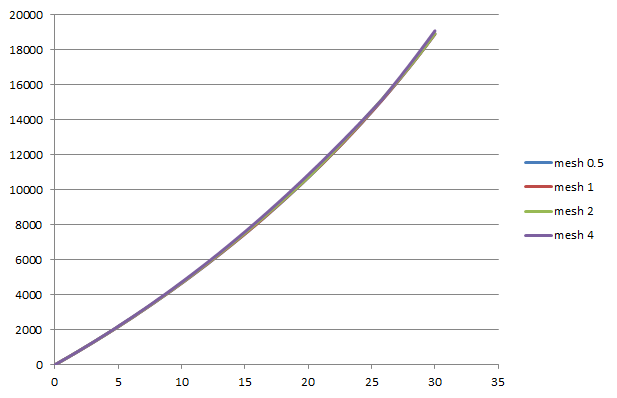
\includegraphics[width=\textwidth]{comparaison_mesh}
	\caption{Réponse force-déplacement de la butée pour différentes tailles de maille.}
	\label{fig1}
\end{figure}


On constate à première vue aucune différence entre les différentes courbes et par conséquent entre les différents maillages. Quand on zoom pour regarder précisément la valeur maximale de la force de réaction pour une flèche de 30cm, comme sur la figure~\ref{fig2}, on constate une lègère différence de 150XXX, c'est-à-dire de 0.8\%, entre un maillage de 4 et 2cm. Un pour un paramètre de maille plus fin, la valeur maximale de la force de réaction converge vers une même valeur.

\begin{figure}[!h]
	\centering
	%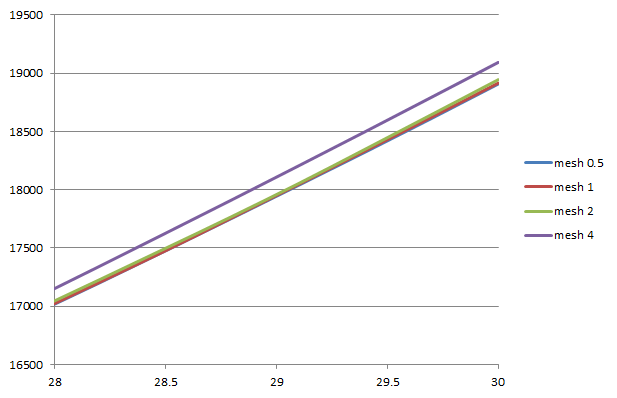
\includegraphics[width=\textwidth]{comparaison_mesh_zoom}
	\caption{Réponse force-déplacement de la butée pour différentes tailles de maille - Zoom.}
	\label{fig2}
\end{figure}

La finesse du maillage n'a donc que très peu d'influence dans notre étude de la raideur de la butée. Un maillage de base d'élements de 2cm de largeur a été cependant choisi pour limiter le temps de calcul, bien qu'un maillage plus fin soit nécessaire dans beaucoup des modèles proposés où le contact avec les pièces additionneles est crutial.


\section{Butée initiale}

L'objectif de cette première partie de l'étude est de décrire le comportement en compression d'une butée offshore en élastomère libre de tout autre élément ou contrainte, afin de rendre compte de la raideur axiale de la pièce et ainsi pouvoir la comparer avec la raideur des autres modèles présentés dans la suite de l'étude.

La forme et le matériau de la butée ainsi que le déplacement imposé à ce dernier ont été décrits dans l'approche du problème. Les élements du maillage dont en S4R et ont pour paramètre 2mm. L'apparence du maillage initial de la pièce est présentée dans la figure~\ref{fig3}.

\begin{figure}[!h]
	\centering
	%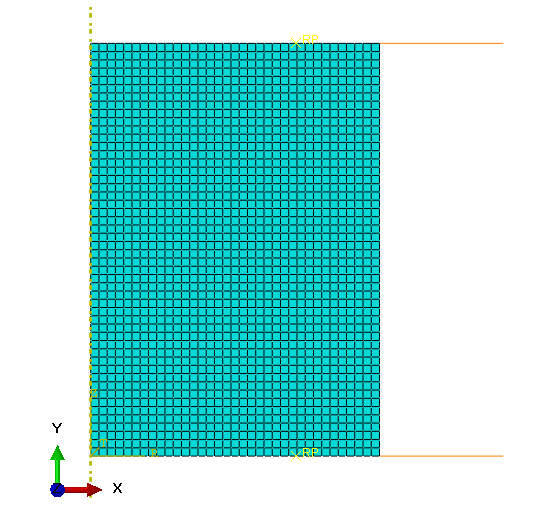
\includegraphics[width=\textwidth]{image_initial_mesh2}
	\caption{Visuel du maillage appliqué à la butée initiale.}
	\label{fig3}
\end{figure}

La figure~\ref{fig4} permet de se rendre compte de l'écrasement subi par la butée. La déformation latérale maximale est de 23\%.

\begin{figure}[!h]
	\centering
	%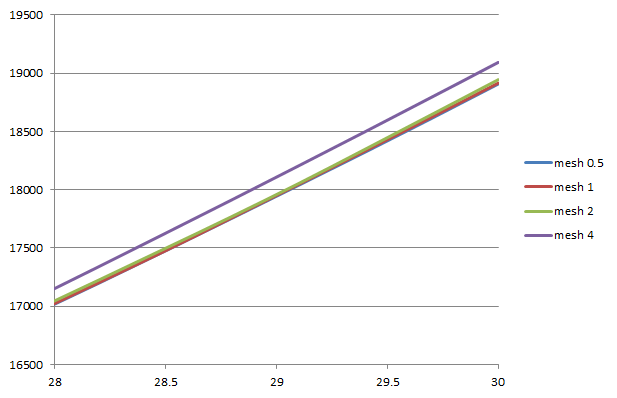
\includegraphics[width=\textwidth]{comparaison_mesh_zoom}
	\caption{Visuel de la butée initiale suite à la compression (déformations Ux affichées).}
	\label{fig4}
\end{figure}

La réponse force-déplacement de la butée initiale est affichée dans la figure~\ref{fig5}

\begin{figure}[!h]
	\centering
	%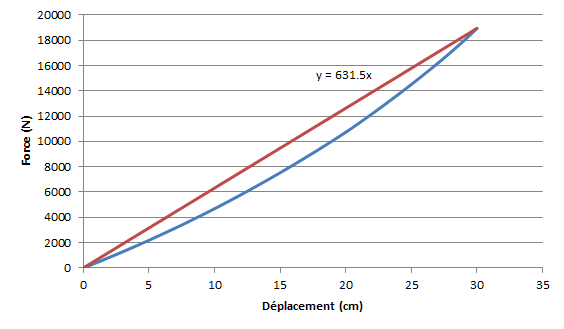
\includegraphics[width=\textwidth]{uf_initial_mesh2}
	\caption{Réponse force-déplacement de la butée initiale.}
	\label{fig5}
\end{figure}

On obtient donc une raideur de 631N/cm. Cette valeur servira de référence pour la suite de l'étude.


\section{Butée raidie par des lamelles}

Une première modification apportée à la butée initiale en vue de quadrupler sa raideur va consister à inister des lamelles horizontales réparties régulièrement sur la hauteur de la pièce avec deux diamètres différents: des lamelles circulaires du même diamètre que la butée en élastomère avant sa compression, que l'on nommera "lamelles imbriquées" et des lamelles avec un diamètre plus élevé que l'on nommera "lamelles étendues". On étudiera ce modèle renforcé d'une, deux et trois lamelles et on regardera l'influence du diamètre de ces dernières sur la raideur finale de la butée. Enfin, nous verrons que l'épaisseur de ces lamelles horizontales a peu d'influence sur les résultats.

\subsection{Lamelles imbriquées}

Un premier modèle d'insertion de lamelles horizontales circulaires de même rayon que l'élastomère à l'état initial (70cm) a été construit sur \abaqus. Il a consisté à diviser la \textit{part} "Butée" en 3 différentes \textit{part}, c'est-à-dire en insérant un élément au milieu des deux autres éléments constituants la butéee en élastomère.

L'épaisseur de la lamelle a été fixée arbitrairement\footnote{Enfin, -"arbitrairement"-, avec la prise en considération d'un certain ordre de grandeur relatif au matériau, tout de même.} à 0.5cm pour commencer les simulations. Cette valeur n'étant pas incohérente vis-à-vis des résultats dans la suite, elle a été conservée. Dans la partie XXXX, il sera montré que l'épaisseur a peu d'influence sur le résultat, et sachant que cette butée à une application industrielle, un plus faible dimensionnement pour une plus faible masse sera favorisé. 
Les figures~\ref{fig6} et~\ref{fig7} présentent l'aspect de la butée avant la simulation de compression, respectivements avec les propriétés de matériau et avec un maillage de taille 2cm appliqué.

\begin{figure}[htbp]
	\begin{minipage}[c]{.45\linewidth}
	\begin{center}
	%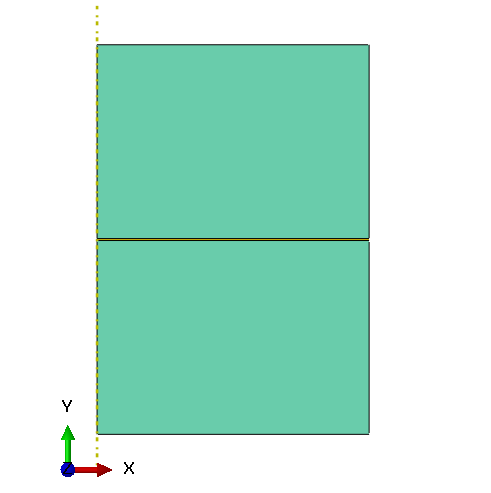
\includegraphics[width=1.2\textwidth]{image_1lamelle_property}
	\caption{Visuel des propriétes appliquées à la butée avec une lamelle imbriquée.}
	\label{fig6}
	\end{center}
	\end{minipage}
	\hfill
	\begin{minipage}[c]{.45\linewidth}
	\begin{center}
	%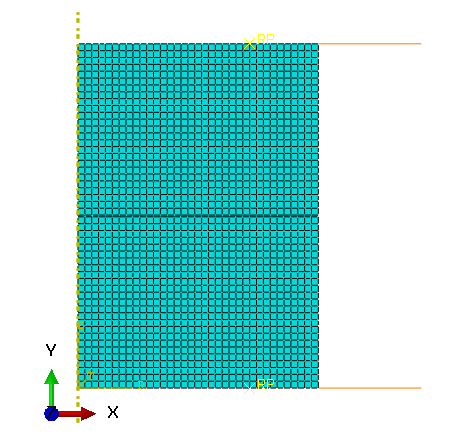
\includegraphics[width=1.2\textwidth]{image_1lamelle_mesh}
	\caption{Visuel du maillage appliqué à la butée avec une lamelle imbriquée.}
	\label{fig7}
	\end{center}
	\end{minipage}
\end{figure}

La lamelle ayant été insérée par une partition de la \textit{part} "Butée", elle est par défintion entièrement liée sur sa surface supérieure et inférieure aux deux parties d'élastomères. Ainsi, aucune propriété de contact surfacique supplémentaire n'a été attribuée au contact entre la lamelle et l'élastomère. Seule une propriété d'auto-contact (\textit{self-contact} dans \abaqus) définie par un contact normal dur (\textit{hard}) et un contact tangentiel \textit{rough} a été ajouté à la surface extérieure de la partie en elastomère. 

La figure~\ref{fig8} présente l'aspect de la butée raidie avec une lamelle suite à la compression.

\begin{figure}[!h]
	\centering
	%\includegraphics[width=\textwidth]{screen_1lamelle_mesh2_u1}
	\caption{Visuel de la butée avec une lamelle imbriquée suite à la compression (déformations Ux affichées).}
	\label{fig8}
\end{figure}

La courbe de la figure~\ref{fig9} correspond à la réponse force-déplacement de la butée raidie avec une lamelle. On constate que la raideur est passée de 631N à 1053N avec l'ajout d'une lamelle, c'est-à-dire une augmentation de 67\%. Cette solution est donc encore loin des 300\% nécessaires pour valider la condition d'augmentation de la raideur.

\begin{figure}[!h]
	\centering
	%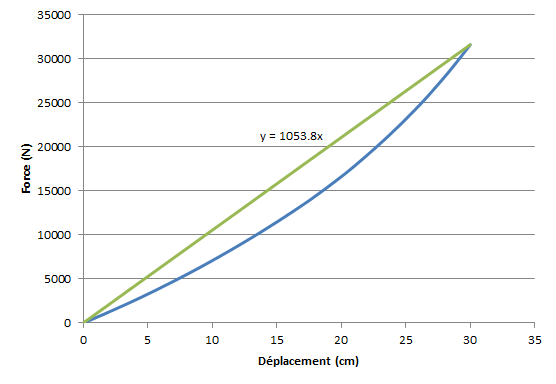
\includegraphics[width=\textwidth]{uf_1lamelle_mesh2}
	\caption{Réponse force-déplacement de la butée avec une lamelle imbriquée.}
	\label{fig9}
\end{figure}

L'étude de cette solution s'est poursuivie avec l'insertion d'une seconde lamelle dans la butée. Des paramètres de contact identiques à ceux présentés précédemment ont été définis. La figure~\ref{fig10} présente l'aspect maillé de la butée avant la simulation de compression, et la figure~\ref{fig11} en donne l'aspect après.

\begin{figure}[!h]
	\centering
	%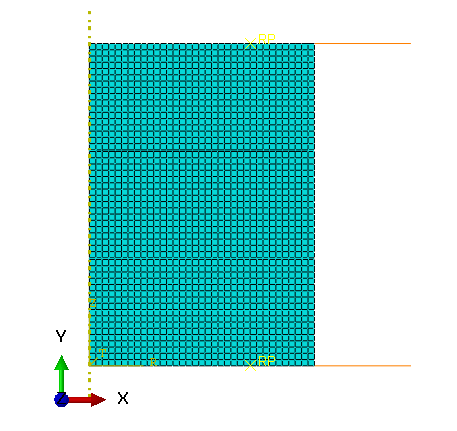
\includegraphics[width=\textwidth]{image_2lamelles_mesh}
	\caption{Visuel du maillage appliqué à la butée avec deux lamelles imbriquées.}
	\label{fig10}
\end{figure}

\begin{figure}[!h]
	\centering
	%\includegraphics[width=\textwidth]{screen_2lamelles_mesh2_u1}
	\caption{Visuel de la butée avec deux lamelles imbriquées suite à la compression (déformations Ux affichées).}
	\label{fig11}
\end{figure}

La courbe de la figure~\ref{fig12} indique la valeur de la raideur de cette butée: 1690N. Ceci correspond à une augmentation de 168\% de la raideur par rapport à celle de la butée initiale. Cepandant, cette raideur n'est pas encore suffisante et ainsi cette solution n'est pas validée.
 
\begin{figure}[!h]
	\centering
	%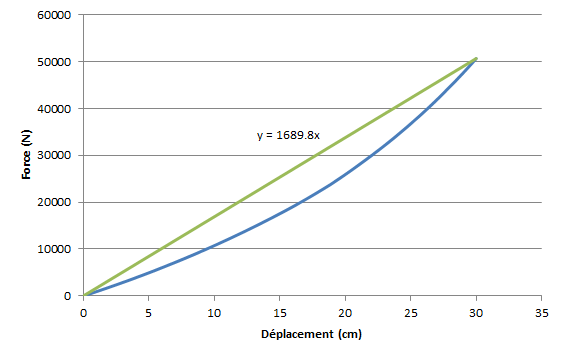
\includegraphics[width=\textwidth]{uf_2lamelles_mesh2}
	\caption{Réponse force-déplacement de la butée avec deux lamelles imbriquées.}
	\label{fig12}
\end{figure}

Il s'agit ainsi d'ajouter encore une troisième lamelle dans le modèle pour espérer atteindre la valeur de raideur prescrite, c'est-à-dire quatre fois plus grande que celle du modèle initial de 631N, soit environ 2500N. La figure~\ref{fig13} présente l'aspect maillé de la butée avec trois lamelles avant la simulation de compression, et on constatera que la taille d'élément a due être affinée à 1cm pour le calcul, et la figure~\ref{fig14} en donne l'aspect après la simulation.

\begin{figure}[!h]
	\centering
	%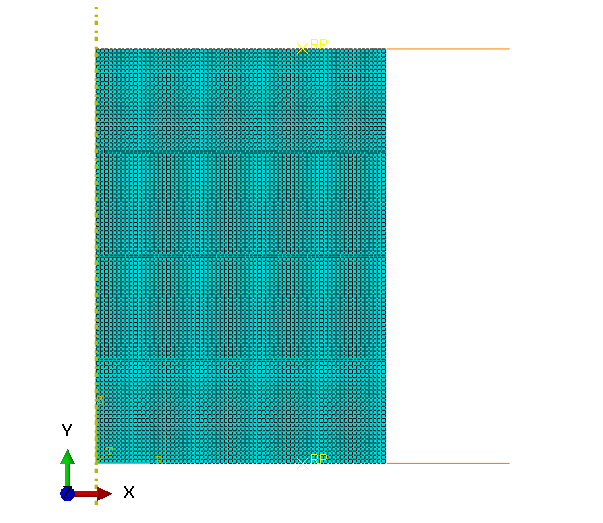
\includegraphics[width=\textwidth]{image_3lamelles_mesh}
	\caption{Visuel du maillage appliqué à la butée avec trois lamelles imbriquées.}
	\label{fig13}
\end{figure}

\begin{figure}[!h]
	\centering
	%\includegraphics[width=\textwidth]{screen_2lamelles_mesh2_u1}
	\caption{Visuel de la butée avec trois lamelles imbriquées suite à la compression (déformations Ux affichées).}
	\label{fig14}
\end{figure}

La figure~\ref{fig15} présente la réponse force-déplacement de la butée offshore avec 3 lamelles imbriquées et indique une valeur de raideur de 2320N. Ceci correspond à une augmentation de 268\% de la raideur par rapport à celle de la butée initiale. Malheureusement, cette solution n'atteint toujours pas l'objectif de 300\%.
 
\begin{figure}[!h]
	\centering
	%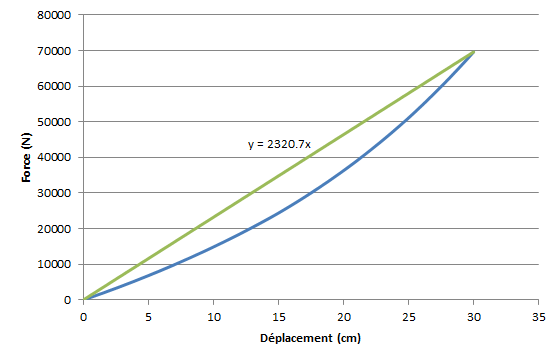
\includegraphics[width=\textwidth]{uf_3lamelles_mesh1}
	\caption{Réponse force-déplacement de la butée avec trois lamelles imbriquées.}
	\label{fig15}
\end{figure}

\subsection{Lamelles étendues}
%changement des paramètres de contact -> penalty avec k=10
Il a été montré dans la partie précédente que même avec l'insertion de 3 lamelles fines (équitablement réparties sur la hauteur) à la butée, le critère de quadruplement de la raideur de la butée initiale n'est pas tout à fait validé. La figure~\ref{fig16} présente une vue rapprochée de l'auto-contact qui s'effectue au niveau des lamelles.

\begin{figure}[!h]
	\centering
	%\includegraphics[width=\textwidth]{screen_1lamelle_mesh2_u1_zoom}
	\caption{Visuel du contact qui s'effectue au niveau des lamelles.}
	\label{fig16}
\end{figure}

Sur cette figure on constate que l'élastomère se déforme au-delà de l'horizontale formé par la face supérieure (ou inférieure) de la lamelle. C'est ensuite le contact avec l'autre partie d'élastomère qui l'empèche de se déformer au-delà du plan médian de la lamelle. Dans notre cas, la lamelle est relativement fine, ce qui implique que l'élastomère ne peut se déformer verticalement que sur 0.25cm. Pourtant, ce detail semble avoir son importance.

Ainsi, un second modèle de butée raidie par insertion de lamelles horizontales est introduit. Il se distingue du premier par le diamètre des lamelles; ici, les lamelles auront un rayon de 80cm, soit 10cm de plus que le rayon de l'élastomère à l'instant initial. Théoriquement, la raideur devrait être légèrement augmentée par l'absence de delta de déformation verticale.

Les pièces ont donc été dimensionnées séparément sur \abaqus, puis ajoutées ensemble. La figure~\ref{fig17} en donne un aspect visuel pour une lamelle étendue insérée. Le contact entre les lamelles et l'élastomère ainsi que l'auto-contact ont été définis par un contact normal \textit{hard} et un contact tangentiel \textit{penalty}.

\begin{figure}[!h]
	\centering
	%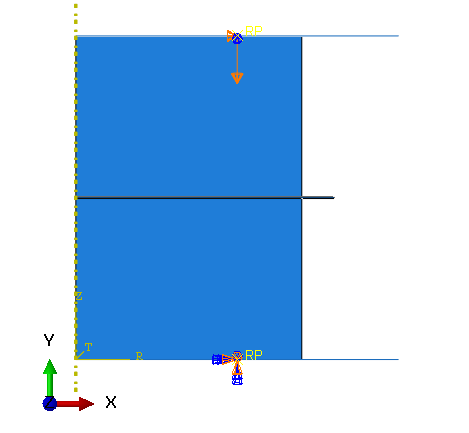
\includegraphics[width=\textwidth]{image_1lamelle_large_load}
	\caption{Visuel de la butée avec une lamelle étendue avant la compression.}
	\label{fig17}
\end{figure}

La figure~\ref{fig18} présente l'aspect de la butée raidie avec une lamelle suite à la compression.

\begin{figure}[!h]
	\centering
	%\includegraphics[width=\textwidth]{screen_1lamelle_large_mesh2_u1}
	\caption{Visuel de la butée avec une lamelle étendue suite à la compression (déformations Ux affichées).}
	\label{fig18}
\end{figure}

On constate d'après les courbes de la figure\ref{fig19} que la raideur n'est passée que de 1053N à 1060N avec l'ajout d'une lamelle étendue, c'est-à-dire une augmentation de moins d'1\%. Si cette faible influence du diamètre de la lamelle se confirme, il est à craindre que cette solution ne suffise toujours pas à valider le critère.

\begin{figure}[!h]
	\centering
	%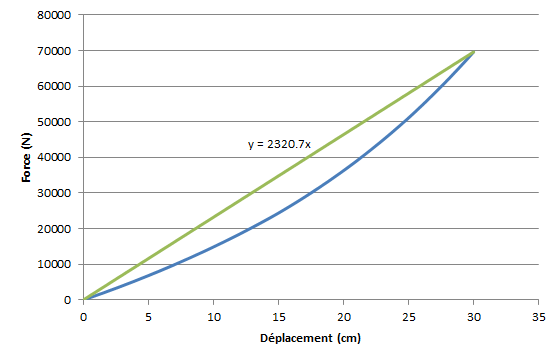
\includegraphics[width=\textwidth]{uf_1lamelle_large_mesh1}
	\caption{Réponse force-déplacement de la butée avec une lamelle étendue.}
	\label{fig19}
\end{figure}

Les figures~\ref{fig20} et~\ref{fig21} donnent un aspect visuel de la déformation suite à la compression des butées avec deux et trois lamelles étendues respectivement.

\begin{figure}[htbp]
	\begin{minipage}[c]{.45\linewidth}
	\begin{center}
	%\includegraphics[width=1.2\textwidth]{screen_2lamelles_large_mesh1_u1}
	\caption{Visuel de la déformation subie par la butée avec deux lamelles étendues.}
	\label{fig20}
	\end{center}
	\end{minipage}
	\hfill
	\begin{minipage}[c]{.45\linewidth}
	\begin{center}
	%\includegraphics[width=1.2\textwidth]{screen_3lamelles_large_mesh1_u1}
	\caption{Visuel de la déformation subie par la butée avec trois lamelles étendues.}
	\label{fig21}
	\end{center}
	\end{minipage}
\end{figure}

Les courbes des figures~\ref{fig22} et~\ref{fig23} représentent les réponses force-déplacement associées aux butées avec deux et trois lamelles.

\begin{figure}[htbp]
	\begin{minipage}[c]{.45\linewidth}
	\begin{center}
	%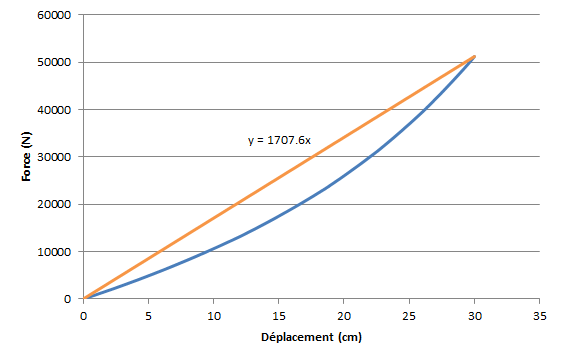
\includegraphics[width=1.2\textwidth]{uf_2lamelles_large_mesh1}
	\caption{Réponse force-déplacement de la butée avec deux lamelles étendues.}
	\label{fig22}
	\end{center}
	\end{minipage}
	\hfill
	\begin{minipage}[c]{.45\linewidth}
	\begin{center}
	%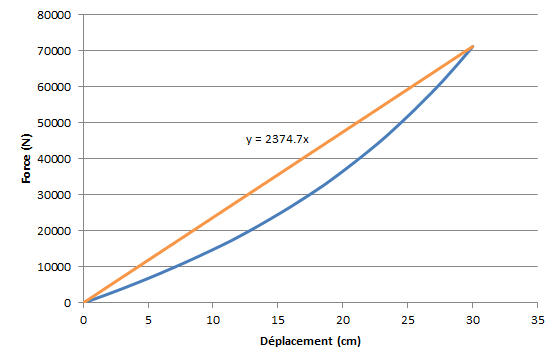
\includegraphics[width=1.2\textwidth]{uf_3lamelles_large_mesh1}
	\caption{Réponse force-déplacement de la butée avec trois lamelles étendues.}
	\label{fig23}
	\end{center}
	\end{minipage}
\end{figure}

On constate en effet que pour 2 lamelles étendues, la raideur grimpe à 1708N (1.1\% de plus que pour les lamelles imbriquées) et pour trois lamelles, elle monte à 2375N, ce qui est toujours en deça des 2500N espérés. Ainsi, la solution d'étendre les lamelles au-delà du diamètre de l'élastomère n'était pas idéal, en plus de présenter une augmentation de masse conséquente.

\subsection{Influence de l'épaisseur des lamelles}
%àfaire



\section{Butée raidie par des anneaux}
%constraint coupling entre le point intérieur de la rondelle et le point exterieur de la butée
%self_contact aussi après


\section{Conclusion}

\listoffigures

\begin{thebibliography}{9}
%\bibitem{latexpratique} Christian \textsc{Rolland}. \emph{\LaTeX{} par la pratique}. O'Reilly, 1999.
%\bibitem[label]{cle} Auteur, TITRE, editeur, annee
%\bibitem{label 1}{cle 2}{Auteur 3}{TITRE 4}{editeur 5}{annee 6}
%\bibitem{msc}{mcstest}{MSC}{Nonlinear finite elements analysis of elastomers}{MSC Software}{20XX}
\bibitem{msc} Nonlinear finite elements analysis of elastomers
\bibitem{wiki_MR} https://en.wikipedia.org/wiki/Mooney%E2%80%93Rivlin_solid
% MSC Software, Nonlinear finite elements analysis of elastomers, MSC, 
% CONTACT_SEMINAR page 259
% Mooney Rivlin
%https://en.wikipedia.org/wiki/Mooney%E2%80%93Rivlin_solid
\end{thebibliography}
\end{document}
% TOREAD http://www.continuummechanics.org/mooneyrivlin.html
% TOREAD http://dmm.im.ufrj.br/~liu/Papers/MooneyRivlin.pdf
